\documentclass{article}
  \def\pathToRoot{../../}\usepackage{nag}
\makeatletter
\@ifclassloaded{beamer}{}
{\usepackage[small,compact]{titlesec}}
\makeatother
\usepackage[utf8]{inputenc}
\usepackage[T1]{fontenc}
\usepackage{lmodern}
\usepackage{color}
\usepackage{parskip}
\usepackage{needspace}
\usepackage{microtype}
\usepackage{mathtools}
\usepackage{xifthen}
\usepackage{xpatch}
\usepackage{enumitem}
\usepackage{mdwlist}
\usepackage{bussproofs}
\EnableBpAbbreviations
\usepackage{tabu}
\usepackage{amssymb}
\usepackage{amsmath}
\usepackage{amsthm}
%grober hack, der den groben hack von parskip bei den amsthm sachen korrigiert
\begingroup
    \makeatletter
       \@for\theoremstyle:=definition,remark,plain\do{%
            \expandafter\g@addto@macro\csname th@\theoremstyle\endcsname{%
                        \addtolength\thm@preskip\parskip
             }%
        }
\endgroup
\usepackage[UKenglish]{babel}
\usepackage{xparse}
\usepackage{adjustbox}
\usepackage{geometry}
\usepackage{booktabs}
\usepackage{multicol}
\usepackage{soul}
\usepackage{calc}
\usepackage{textcase}
\usepackage{stmaryrd}
\usepackage{marvosym}
\usepackage{wasysym}
\usepackage{pifont}
\newcommand{\cmark}{\ding{51}}
\newcommand{\xmark}{\ding{55}}
\usepackage{tikz}
\usetikzlibrary{trees, backgrounds, shapes, chains, decorations.text, decorations.pathreplacing, circuits.logic.IEC, patterns, matrix}
\usepackage{tikz-qtree}
\usepackage{tikzsymbols}
\usepackage{fancyvrb}
\usepackage{fancyhdr}
\usepackage{verbatim}
\usepackage[framemethod=tikz]{mdframed}
\usepackage{lastpage}
\usepackage{pgfpages}
\usepackage{csquotes}
\usepackage{longtable}
\usepackage{ragged2e}
%\usepackage{stackengine}
\usepackage{censor}
\usepackage{expl3}
\usepackage{multirow}
\usepackage{hyperref}
\usepackage{environ}


% Package for Cateogry diagrams:

\usepackage{tikz-cd}



\ifcsdef{labelenumi}{
\renewcommand{\labelenumi}{(\alph{enumi})}
\renewcommand{\labelenumii}{(\roman{enumii})}
}{}

\input{\pathToRoot headers/definitions}



\tikzset{
    normal/.style={draw, semithick},
    n/.style={style=normal, circle, inner sep=1mm, minimum size=8mm},
    l/.style={style=normal, rounded corners=1mm, inner sep=1mm, minimum size=6mm},
    e/.style={style=normal, shorten >=1mm, shorten <=1mm, ->, >=stealth},
    syntax/.style={style=normal, ellipse, minimum height=6mm, minimum width=8mm}, % nodes in syntax trees
    inner/.style={style=normal, minimum size=4mm}, % inner leaves or root in normal trees
    leaf/.style={style=normal, circle, minimum size=4mm}, % leaves in normal trees
    te/.style={style=normal}, % edges in a tree
    be/.style={style=e, dashed} % binding edge
}

\newcommand{\syntaxtree}[1]{ % DEPRECATED - use tikzsyntaxtree
    \begin{tikzpicture}[baseline=(current bounding box.north)]
        \tikzset{grow=down}
        \tikzset{every node/.style={syntax}}
        \tikzset{edge from parent/.style=
            {te,
                edge from parent path={(\tikzparentnode) -- (\tikzchildnode)}}}
        \Tree #1
    \end{tikzpicture}
}

\newenvironment{tikzsyntaxtree}[1][]{
    \begin{tikzpicture}[baseline=(current bounding box.north), #1]
    \tikzset{grow=down}
    \tikzset{every tree node/.style={syntax}}
    \tikzset{edge from parent/.style={te, edge from parent path={(\tikzparentnode) -- (\tikzchildnode)}}}
}{
    \end{tikzpicture}
}


\newcommand{\DisplayScaledProof}{\maxsizebox{\linewidth}{!}{\DisplayProof}}
\newcommand{\DisplayTopProof}{\adjustbox{valign=t}{\DisplayProof}}
\newcommand{\DisplayScaledTopProof}{\adjustbox{valign=t}{\maxsizebox{\linewidth}{!}{\DisplayProof}}}


\newcolumntype{P}[1]{>{\RaggedRight\hspace{0pt}}p{#1}}

\newenvironment{prooftable}
{
    \begin{longtable}{>{\footnotesize}p{0.33\textwidth}>{\footnotesize}p{0.33\textwidth}|>{\footnotesize}P{0.15\textwidth}}
    \normalsize Textbeweis & \normalsize Erklärungen & \normalsize Schlussregel\\\hline
    \endhead
}
{
    \end{longtable}
}


\theoremstyle{definition}
\newtheorem*{definition*}{Definition} % Definition ohne Nummer
\newtheorem*{inferenceRule*}{Schlussregel}

  \usepackage{microtype}
  
  
  \graphicspath{{graphics/}}
  
  
  \usepackage{mathpartir}
  \theoremstyle{plain}
  \newtheorem{lemma}{Lemma}
  \newtheorem{theorem}{Theorem}
  \theoremstyle{definition}
  \newtheorem{definition}{Definition}
  
  
  \usetikzlibrary{fit}
  \usetikzlibrary{knots}
  
  \tikzstyle{morphism}=[draw, minimum size=0.5cm, semithick]
  \tikzstyle{phantom morphism}=[minimum size=0.5cm]
  \tikzstyle{object}=[semithick]
  
  
  \begin{document}
  \title{The Graphical Calculus for Monoidal Categories}
  \author{Felix Rech}
  \maketitle
  
  
  In this chapter, we will talk about a certain class of categories that have a binary operation on objects.
  We call them monoidal categories because they combine the concept of a category and that of a monoid.
  Our central goal is to introduce a \emph{graphical calculus} for the construction of morphisms in such categories.
  This calculus hides non-essential details of constructions.
  Hence it is easy to understand what a morphism does and to decide whether two morphisms are equal or not.
  To illustrate this, assume that we have four morphisms $B
  \xrightarrow{f, g} B$, $C \xrightarrow{h} B$ and $A \xrightarrow{k} B \times C$ in the category of sets.
  Can you tell if the following equation is valid?
  \[ \rounddd{f \times (g \of h)} \of k = (1 \times f) \of \rounddd{(g \times h) \of k} \]
  The answer is that in general the equation does not hold.
  But at first glance, this is not obvious, although both constructions are rather simple.
  Now take a look at this graphical representation of the equation:
  \[
    \vcenter{ \hbox{ 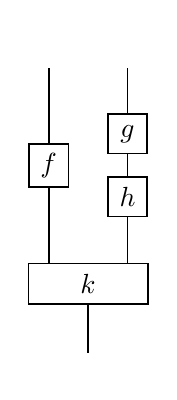
\begin{tikzpicture}
          \node[phantom morphism] (out1) at (0, 4) {};
          \node[morphism] (f) at (0, 2.5) {$f$};
          \node[phantom morphism] (out2) at (1, 4) {};
          \node[morphism] (g) at (1, 2.9) {$g$};
          \node[morphism] (h) at (1, 2.1) {$h$};
          \node[phantom morphism] (k_left) at (0, 1) {};
          \node[phantom morphism] (k_right) at (1, 1) {};
          \node[morphism, fit=(k_left) (k_right), inner sep=0, ] (k) {};
          \node at (k) {$k$};
          \node (in) at (0.5, 0) {};
  
          \draw[object] (f) to (out1);
          \draw[object] (k_left) to (f);
          \draw[object] (g) to (out2);
          \draw[object] (h) to (g);
          \draw[object] (k_right) to (h);
          \draw[object] (in) to (k);
        \end{tikzpicture}}}
    =
    \vcenter{ \hbox{ 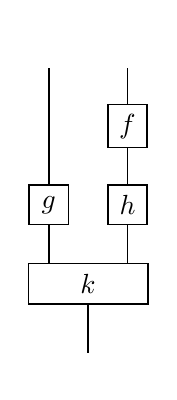
\begin{tikzpicture}
          \node[phantom morphism] (out1) at (0, 4) {};
          \node[morphism] (g) at (0, 2) {$g$};
          \node[phantom morphism] (out2) at (1, 4) {};
          \node[morphism] (f) at (1, 3) {$f$};
          \node[morphism] (h) at (1, 2) {$h$};
          \node[phantom morphism] (k_left) at (0, 1) {};
          \node[phantom morphism] (k_right) at (1, 1) {};
          \node[morphism, fit=(k_left) (k_right), inner sep=0, ] (k) {};
          \node at (k) {$k$};
          \node (in) at (0.5, 0) {};
  
          \draw[object] (g) to (out1);
          \draw[object] (k_left) to (g);
          \draw[object] (f) to (out2);
          \draw[object] (h) to (f);
          \draw[object] (k_right) to (h);
          \draw[object] (in) to (k);
        \end{tikzpicture}}}.
  \]
  Each side of the equation can be read like the drawing of a circuit with outputs at the top and inputs at the bottom.
  Wires and boxes that run in parallel, stand for the Cartesian product of objects and morphisms respectively.
  It is okay if you do not immediately understand how this notation works.
  It will become clear over the next few pages.
  The important message is that circuit-like drawings of morphisms are often easier to understand and compare than algebraic expressions.
  
  In our example above we used the category of sets with the Cartesian product as the binary operation.
  For the circuit metaphor, this means that inputs and outputs of the circuit consist of signals on all input or output wires simultaneously.
  We could also use the disjoint union as operation, in which case inputs and outputs would consist of a single signal on one of those wires.
  Another option is to use the category of relations with the Cartesian product.
  If we interpret relations as non-deterministic functions then this yields non-deterministic circuits.
  In fact, we could do this with most categories and binary operations that we normally encounter.
  In the end of this chapter, you will see that circuits are just the start and that we can extend or generalize the calculus to represent more concepts in this powerful way.
  
  This chapter is based on unpublished lecture notes about categorical quantum mechanics by Daniel Marsden and Jamie Vicary from 2016.
  For more details, background and omitted proofs, we refer to those lecture notes or an older version by Chris Heunen and Jamie Vicary~\cite{heunen2015cqm}.
  
  
  \section{Graphical Calculus for General Categories}
  
  We will now start with the introduction of those components of the graphical calculus that can be applied for all categories.
  We draw objects as vertical lines that we also refer to as wires and morphisms as boxes.
  If there is a morphism $A \xrightarrow{f} B$ then we draw it as a box with an output wire at the top and an input wire at the bottom:
  \[ \includegraphics{morphism}. \]
  Often we omit labels on object and morphisms if they are not essential.
  
  For two morphisms $A \xrightarrow{f} B$ and $B \xrightarrow{g} C$, we use the output wire of the $f$-box as input wire to the $g$-box to denote the composition $g \of f$:
  \[ \includegraphics{vertical_composition}. \]
  
  So far this is basically the same as the algebraic notation that we are used to, except that we read it top to bottom instead of left to right.
  In the same way as we can do it with the algebraic notation, we usually omit parentheses and do not draw identity morphisms.
  
  
  \section{Monoidal Categories}
  
  We have defined what it means to connect multiple morphisms in a chain, but how do we combine morphisms in parallel?
  As mentioned earlier, we need a binary operation on objects for that which should also operate on morphisms.
  Hence it seems reasonable to require it to be a functor.
  We will call it tensor product because the tensor product of vector spaces is a prominent example.
  For our purposes, we need some minimal structure on such a vector product.
  Inspired by the definition of a monoid, we require associativity and a neutral element that we call unit.
  This leads us to the definition of a strict monoidal category.
  
  \begin{definition}
    A \demph{strict monoidal category} is a category $C$ with the following:
    \begin{description}
    \item[Tensor product:] A functor $\otimes : C \times C \to C$
    \item[Unit object:] An object $I \in \ob(C)$
    \item[Associativity:] An equality $(A \otimes B) \otimes C = A \otimes (B \otimes C)$ for all objects $A$, $B$ and $C$
    \item[Left unit law:] An equality $I \otimes A = A$ for all objects $A$
    \item[Right unit law:] An equality $A \otimes I = A$ for all objects $A$
    \end{description}
  \end{definition}
  
  Our original example, that served as motivation for this definition, was the category of sets with the Cartesian product as the tensor product.
  If we check the details, however, we see that it does not actually satisfy the definition because associativity and the unit laws hold only up to isomorphism.
  To admit this, we define monoidal categories as a generalization of strict monoidal categories.
  
  \begin{definition}
    A \demph{monoidal category} is a category $C$ with the following:
    \begin{description}
    \item[Tensor product:] A functor $\otimes : C \times C \to C$
    \item[Unit object:] An object $I \in \ob(C)$
    \item[Associator:] A natural isomorphism $(A \otimes B) \otimes C \xrightarrow{\smash{\alpha_{A, B, C}}} A \otimes (B \otimes C)$ for all objects $A$, $B$ and $C$
    \item[Left unitor:] A natural isomorphism $I \otimes A \xrightarrow{\smash{\lambda_A}} A$ for all objects $A$
    \item[Right unitor:] A natural isomorphism $A \otimes I \xrightarrow{\rho_A} A$ for all objects $A$
    \end{description}
  
    Those have to satisfy the \demph{triangle} and \demph{pentagon equalities}:
    \[ \begin{adjustbox}{max totalsize={\textwidth}{\textheight}, center}
      \begin{tikzcd}[column sep=0]
        (A \otimes I) \otimes B
        \arrow[dr, "\rho_A \otimes 1_B"']
        \arrow[rr, "\alpha_{A, I, B}"] &&
        A \otimes (I \otimes B)
        \arrow[dl, "1_A \otimes \lambda_B"] \\
        %
        & A \otimes B
      \end{tikzcd}
      \hspace{1em}
      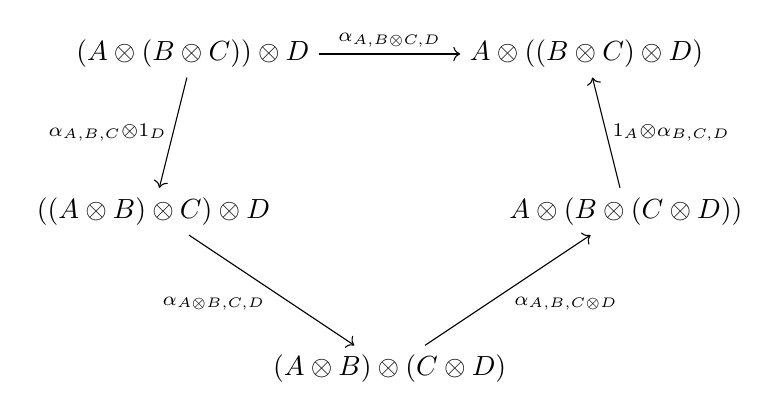
\begin{tikzpicture}[commutative diagrams/every diagram]
        \node (S) at (0, -2)
        {$(A \otimes B) \otimes (C \otimes D)$};
        \node (E) at (3, 0)
        {$A \otimes (B \otimes (C \otimes D))$};
        \node (NE) at (2.5, 2)
        {$A \otimes ((B \otimes C) \otimes D)$};
        \node (NW) at (-2.5, 2)
        {$(A \otimes (B \otimes C)) \otimes D$};
        \node (W) at (-3, 0)
        {$((A \otimes B) \otimes C) \otimes D$};
  
        \draw[commutative diagrams/.cd, every arrow, every label]
        (NW) edge node[anchor=east] {$\alpha_{A, B, C} \otimes 1_D$} (W)
        (W) edge node[anchor=north east] {$\alpha_{A \otimes B, C, D}$} (S)
        (S) edge node[anchor=north west] {$\alpha_{A, B, C \otimes D}$} (E)
        (E) edge node[anchor=west] {$1_A \otimes \alpha_{B, C, D}$} (NE)
        (NW) edge node {$\alpha_{A, B \otimes C, D}$} (NE);
      \end{tikzpicture}
    \end{adjustbox}. \]
  \end{definition}
  
  It is not necessary that you understand the triangle and pentagon equalities.
  The only reason why we have them is to obtain the following coherence property.
  
  \begin{theorem}[Coherence for monoidal categories]
    Given the data of a monoidal category, if the pentagon and triangle equations hold, then any well-typed equation built only from $\lambda$, $\rho$, $\alpha$ and their inverses holds.
  \end{theorem}
  
  An example for the coherence property is the equation $\lambda_I = \rho_I$ which would not follow without the triangle and pentagon equalities.
  Other examples are the triangle and pentagon equations themselves.
  Of course, the statement of the theorem is imprecise because we didn't define what it means for an equation to be well-typed.
  For a counterexample suppose that there is an object $A$ that satisfies the equality $A = (A \otimes A) \otimes A$.
  Then we have morphisms $1_A : A \to A$ and $\alpha_{A, A, A} : A \to A$ and we can write down the equation $1_A = \alpha_{A, A, A}$.
  But this equation is not well-typed in our terms because it uses the extra knowledge about $A$.
  Roughly speaking, an equation is well-typed if it makes sense in every monoidal category and for every choice of objects.
  
  
  \section{Graphical Calculus for Monoidal Categories}
  
  From now on we will talk about monoidal categories and extend our graphical calculus to express the tensor product of morphisms as parallel combination.
  If we have two morphisms $f : A \to B$ and $g : C \to D$, then we write them side-by-side in the graphical representation to denote the tensor product $f \otimes g$:
  \[ \includegraphics{horizontal_composition}. \]
  Usually, we do not draw the unit object or any parentheses for this parallel combination, which is justified by associativity, the unit laws and the following interchange law.
  
  \begin{theorem}
    In a monoidal category all morphisms $f : A \to B$, $g : B \to C$, $h : D \to E$ and $j : E \to F$ satisfy the equation
    \[ (g \of f) \otimes (j \of h) = (g \otimes j) \of (f \otimes h). \]
    In the graphical calculus this can be written as
    \[ \includegraphics{interchange_law}. \]
  \end{theorem}
  
  We do not draw $\lambda$, $\rho$ and $\alpha$ either:
  \begin{mathpar}
    \includegraphics{lambda} \and
    \includegraphics{rho} \and
    \includegraphics{alpha}.
  \end{mathpar}
  This can be justified by the their naturality and the coherence law.
  The actual proof is complex but you should get a feeling for it if you consider the following properties.
  \begin{itemize}
  \item Naturality allows us to move other morphisms \textit{through} $\lambda$, $\rho$ and $\alpha$.
    Therefore the exact position where we apply those isomorphisms does not matter.
  \item The coherence theorem tells us that the exact selection and combination of those isomorphisms does not matter as long as we fix the input and the output type.
  \end{itemize}
  
  We have given some hints, why the graphical calculus makes sense.
  The next theorem makes this precise and summarizes everything you need to know about the graphical calculus.
  
  \begin{definition}
    Two diagrams are \demph{isotopic} when one can be deformed continuously into the other, keeping the boundaries fixed.
  \end{definition}
  
  This means essentially that we can move things around in one diagram to obtain the other whereby we are not allowed to move one object through another, to move objects outside of the boundary or to remove inputs or outputs from the boundary.
  
  \begin{theorem}[Correctness for monoidal categories]
    A well-typed equation between morphisms in a monoidal category follows from the axioms if and only if it holds in the graphical language up to \textbf{planar} isotopy.
  \end{theorem}
  
  To make this clear, let us first look at a counterexample:
  \[ \includegraphics{simple_counterexample}. \]
  Those two diagrams do not in general represent the same morphism.
  To check if the diagrams are isotopic, take a look at the following schematic representation that contains the boundaries and represents $f$ as a geometric point.
  \[ \includegraphics{simple_counterexample_geometric} \]
  In the plane, we cannot move $f$ from the left half of the diagram to the right half without going through $A$ or leaving the boundary.
  Thus the diagrams are not isotopic and the morphisms are not in general equal.
  
  On the other hand, the following diagrams are obviously isotopic and thus represent the same morphisms.
  
  \[ \includegraphics{simple_example} \]
  
  
  \section{Braided Monoidal Categories}
  
  So far we followed the goal to interpret constructions of circuits as constructions of morphisms in categories and we have nearly achieved that goal, but there is one thing that we can do in circuits but in general not with morphisms in monoidal categories: we cannot \textit{cross wires}:
  There is no general way to construct a morphism $A \otimes B \to B \otimes A$ for arbitrary objects $A$ and $B$.
  We describe monoidal categories that allow us to do this by the following definition.
  
  \begin{definition}
    A \demph{braided monoidal category} is a monoidal category equipped with a natural isomorphism
    \[ A \otimes B \xrightarrow{\sigma_{A, B}} B \otimes A \]
    satisfying the \demph{hexagon equations}:
    \[ \begin{adjustbox}{max totalsize={\textwidth}{\textheight}, center}
      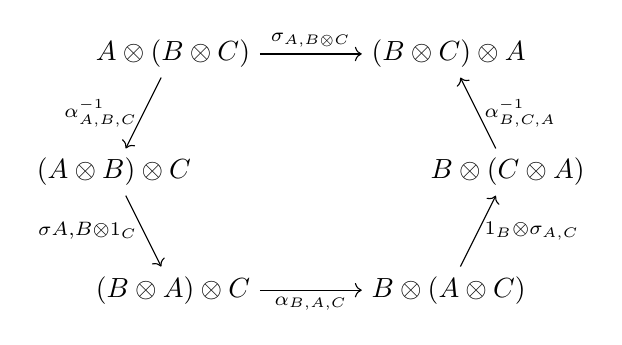
\begin{tikzpicture}[commutative diagrams/every diagram]
        \node (SW) at (-1.75, -1.5)
        {$(B \otimes A) \otimes C$};
        \node (SE) at (1.75, -1.5)
        {$B \otimes (A \otimes C)$};
        \node (E) at (2.5, 0)
        {$B \otimes (C \otimes A)$};
        \node (NE) at (1.75, 1.5)
        {$(B \otimes C) \otimes A$};
        \node (NW) at (-1.75, 1.5)
        {$A \otimes (B \otimes C)$};
        \node (W) at (-2.5, 0)
        {$(A \otimes B) \otimes C$};
  
        \draw[commutative diagrams/.cd, every arrow, every label]
        (NW) edge node[anchor=east] {$\alpha_{A, B, C}^{-1}$} (W)
        (W) edge node[anchor=east] {$\sigma{A, B} \otimes 1_C$} (SW)
        (SW) edge node[anchor=north] {$\alpha_{B, A, C}$} (SE)
        (SE) edge node[anchor=west] {$1_B \otimes \sigma_{A, C}$} (E)
        (E) edge node[anchor=west] {$\alpha_{B, C, A}^{-1}$} (NE)
        (NW) edge node {$\sigma_{A, B \otimes C}$} (NE);
      \end{tikzpicture}
      \hspace{1em}
      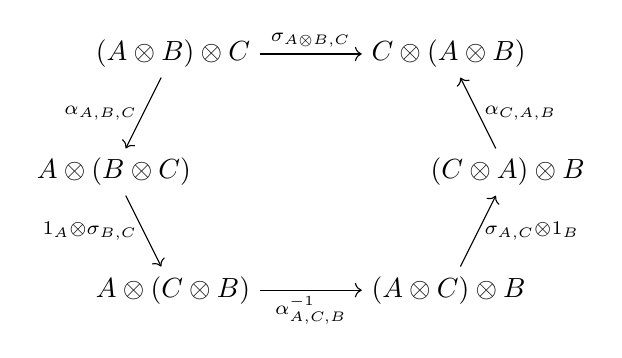
\begin{tikzpicture}[commutative diagrams/every diagram]
        \node (SW) at (-1.75, -1.5)
        {$A \otimes (C \otimes B)$};
        \node (SE) at (1.75, -1.5)
        {$(A \otimes C) \otimes B$};
        \node (E) at (2.5, 0)
        {$(C \otimes A) \otimes B$};
        \node (NE) at (1.75, 1.5)
        {$C \otimes (A \otimes B)$};
        \node (NW) at (-1.75, 1.5)
        {$(A \otimes B) \otimes C$};
        \node (W) at (-2.5, 0)
        {$A \otimes (B \otimes C)$};
  
        \draw[commutative diagrams/.cd, every arrow, every label]
        (NW) edge node[anchor=east] {$\alpha_{A, B, C}$} (W)
        (W) edge node[anchor=east] {$1_A \otimes \sigma_{B, C}$} (SW)
        (SW) edge node[anchor=north] {$\alpha_{A, C, B}^{-1}$} (SE)
        (SE) edge node[anchor=west] {$\sigma_{A, C} \otimes 1_B$} (E)
        (E) edge node[anchor=west] {$\alpha_{C, A, B}$} (NE)
        (NW) edge node {$\sigma_{A \otimes B, C}$} (NE);
      \end{tikzpicture}
    \end{adjustbox}. \]
  \end{definition}
  
  Similar to the triangle and pentagon equations, the hexagon equations have the only purpose to ensure a coherence property that includes not only $\lambda$, $\rho$ and $\alpha$ but also $\sigma$.
  But this time the coherence statement is more complicated.
  For example the equation $1_{A \otimes B} = \sigma_{B, A} \of \sigma_{A, B}$ does not hold in general, even though it is well-typed.
  Again, the coherence property will be important for the correctness of the graphical calculus, but we will not state it here.
  
  We extend the graphical calculus with simple notations for $\sigma$ and its inverse that reflect our intuition of crossing wires:
  \begin{mathpar}
    \overset{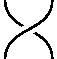
\includegraphics{sigma}}{\sigma} \and
    \overset{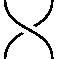
\includegraphics{sigma_inverse}}{\sigma^{-1}}.
  \end{mathpar}
  
  Naturality of $\sigma$ allows to move morphisms through crossings:
  \begin{mathpar}
    \includegraphics{sigma_naturality} \and
    \includegraphics{sigma_inverse_naturality}.
  \end{mathpar}
  
  The fact that $\sigma^{-1}$ is inverse to $\sigma$, means that we can move wires over another:
  \begin{mathpar}
    \includegraphics{sigma_inverse_sigma} \and
    \includegraphics{sigma_sigma_inverse}.
  \end{mathpar}
  
  As you might guess, this together allows us to formulate a new correctness statement that does not consider the graphical representation in the plane but in three-dimensional space.
  
  \begin{theorem}[Correctness for braided monoidal categories]
    A well-typed equation between morphisms in a braided monoidal category follows from the axioms if and only if it holds in the graphical language up to \textbf{spatial} isotopy.
  \end{theorem}
  
  As examples consider the following two pairs of equations between diagrams with their algebraic counterpart.
  
  \[ 
\includegraphics{braiding_example_1} \]
  \[ \alpha \of (\sigma \otimes 1) \of \alpha^{-1} \of (1 \otimes f) \of \rho^{-1}
    = (1 \otimes \sigma^{-1}) \of \alpha \of (f \otimes 1) \of \lambda^{-1} \]
  
  \[ 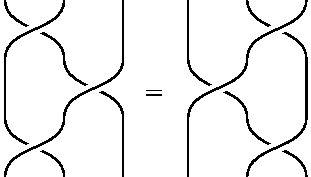
\includegraphics{braiding_example_2} \]
  \[ \alpha \of (\sigma \otimes 1) \of \alpha^{-1} \of (1 \otimes \sigma) \of \alpha \of (\sigma \otimes 1)
    = (1 \otimes \sigma) \of \alpha \of (\sigma \otimes 1) \of \alpha^{-1} \of (1 \otimes \sigma) \of \alpha \]
  
  With our geometric intuition it is obvious that the compared diagrams are isotopic in three-dimensional space and thus the equations hold.
  If you look at the algebraic form however, it becomes much harder to see.
  
  
  \section{Symmetric Monoidal Categories}
  
  You may have noticed that there is one last thing that distinguishes circuits from our constructions in braided monoidal categories.
  In circuits, it does not matter which wire crosses on top.
  In the language of braided monoidal categories this means that $\sigma_{B, A}^{-1} = \sigma_{A, B}$.
   
  \begin{definition}
    A braided monoidal category is \demph{symmetric} when
    \[ \sigma_{B, A}^{-1} = \sigma_{A, B} \]
    for all objects $A$ and $B$.
  \end{definition}
  
  Since we do not need to distinguish between $\sigma$ and $\sigma^{-1}$ anymore, we denote both by the same notation:
  \[ \includegraphics{symmetric_sigma}. \]
  
  The most important consequence of symmetry is that wires can move through each other:
  \[ \includegraphics{symmetry}. \]
  This means that for the correctness statement we can consider four-dimensional isotopy now.
  
  \begin{theorem}[Correctness for symmetric monoidal categories]
    A well-typed equation between morphisms in a symmetric monoidal category follows from the axioms if and only if it holds in the graphical language up to \textbf{four-dimensional} isotopy.
  \end{theorem}
  
  
  \section{Dual Objects}
  
  In this section, we go beyond the circuit metaphor and demonstrate the extensibility and power of the graphical calculus with a new notation for so-called dual objects.
  
  \begin{definition}
    In a monoidal category, an object $L$ is \demph{left-dual} to an object $R$, and $R$ is \demph{right-dual} to $L$, written $L \dashv R$, when there exist
    \begin{itemize}
    \item a \demph{unit} morphism $I \xrightarrow{\eta} R \otimes L$ and
    \item a \demph{counit} morphism $L \otimes R \xrightarrow{\varepsilon} I$
    \end{itemize}
    satisfying the \demph{snake equations}:
    \[ \begin{adjustbox}{max width=\linewidth, center}
      \begin{tikzcd}
        L \arrow[r, "\rho_L^{-1}"] \arrow[d, "1_L"] &
        L \otimes I \arrow[r, "1_L \otimes \eta"] &
        L \otimes (R \otimes L) \arrow[d, "\alpha_{L, R, L}^{-1}"] \\
        %
        L &
        I \otimes L \arrow[l, "\lambda_L"] &
        (L \otimes R) \otimes L \arrow[l, "\varepsilon \otimes 1_L"]
      \end{tikzcd}
      \hspace{1em}
      \begin{tikzcd}
        R \arrow[r, "\lambda_R^{-1}"] \arrow[d, "1_R"] &
        I \otimes R \arrow[r, "\eta \otimes 1_R"] &
        (R \otimes L) \otimes R \arrow[d, "\alpha_{R, L, R}"] \\
        %
        R &
        R \otimes I \arrow[l, "\rho_R"] &
        R \otimes (L \otimes R) \arrow[l, "1_R \otimes \varepsilon"]
      \end{tikzcd}.
    \end{adjustbox} \]
  \end{definition}
  
  To make it obvious if we talk about a left or right dual, we indicate this by an upward or downward arrow respectively:
  \begin{mathpar}
    \includegraphics{left_dual} \and
    \includegraphics{right_dual}.
  \end{mathpar}
  
  For the unit and counit we introduce a special notation:
  \begin{mathpar}
    \overset{\includegraphics{unit}}{\lower 3ex \hbox{\centering unit}} \and
    \overset{\includegraphics{counit}}{\lower 3ex \hbox{\centering counit}}.
  \end{mathpar}
  We say that we can bend wires now.
  With this notation the snake equations take a very simple form:
  \[ \includegraphics{snake_equations}. \]
  They let us straighten arbitrarily bent wires.
  
  We will now present three proofs of basic properties of dual objects to demonstrate how the graphical calculus can make things simple and clear.
  
  \begin{lemma} 
    The left- and right-dual of an object are unique up to isomorphism.
  \end{lemma}
  \begin{proof}
    We show only that the right-dual is unique.
    Assume that $R$ and $R'$ are both right-dual to $L$.
    For convenience, we use the bent-wire notation for both.
    Then we can define morphisms between $R$ and $R'$ by
    \[ \includegraphics{dual_unique}. \]
    From the snake equations, it is easy to see that those are mutually inverse.
    Thus $R' \simeq R$.
  \end{proof}
  
  \begin{lemma}
    The unit of a duality determines the counit and vice-versa.
  \end{lemma}
  \begin{proof}
    We show only that the unit determines the counit.
    The other direction is similar.
    Assume that we have a duality $L \dashv R$ with unit $\eta$ and counit $\varepsilon$ and we have another duality $L \dashv R$, also with unit $\eta$ but with counit $\varepsilon'$.
    Then we have the equality
    \[
      \vcenter{ \hbox{ 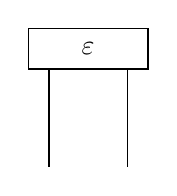
\begin{tikzpicture}
        \node[phantom morphism] (epsilon_left) at (0, 1) {};
        \node[phantom morphism] (epsilon_right) at (1, 1) {};
        \node[morphism, fit=(epsilon_left) (epsilon_right), inner sep=0] (epsilon) {};
        \node at (epsilon) {$\varepsilon$};
  
        \coordinate (in1) at (0, -0.5);
        \coordinate (in2) at (1, -0.5);
        \draw[object] (in1) to (epsilon_left);
        \draw[object] (in2) to (epsilon_right);
      \end{tikzpicture} } }
      =
      \vcenter{ \hbox{ 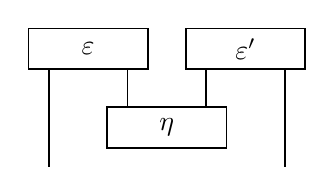
\begin{tikzpicture}
        \node[phantom morphism] (epsilon_left) at (0, 1) {};
        \node[phantom morphism] (epsilon_right) at (1, 1) {};
        \node[morphism, fit=(epsilon_left) (epsilon_right), inner sep=0] (epsilon) {};
        \node at (epsilon) {$\varepsilon$};
  
        \node[phantom morphism] (eta_left) at (1, 0) {};
        \node[phantom morphism] (eta_right) at (2, 0) {};
        \node[morphism, fit=(eta_left) (eta_right), inner sep=0] (eta) {};
        \node at (eta) {$\eta$};
  
        \node[phantom morphism] (epsilon'_left) at (2, 1) {};
        \node[phantom morphism] (epsilon'_right) at (3, 1) {};
        \node[morphism, fit=(epsilon'_left) (epsilon'_right), inner sep=0] (epsilon') {};
        \node at (epsilon') {$\varepsilon'$};
  
        \coordinate (in1) at (0, -0.5);
        \coordinate (in2) at (3, -0.5);
        \draw[object] (in1) to (epsilon_left);
        \draw[object] (eta_left) to (epsilon_right);
        \draw[object] (eta_right) to (epsilon'_left);
        \draw[object] (in2) to (epsilon'_right);
      \end{tikzpicture} } }
      =
      \vcenter{ \hbox{ 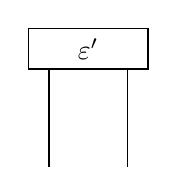
\begin{tikzpicture}
        \node[phantom morphism] (epsilon'_left) at (2, 1) {};
        \node[phantom morphism] (epsilon'_right) at (3, 1) {};
        \node[morphism, fit=(epsilon'_left) (epsilon'_right), inner sep=0] (epsilon') {};
        \node at (epsilon') {$\varepsilon'$};
  
        \coordinate (in1) at (2, -0.5);
        \coordinate (in2) at (3, -0.5);
        \draw[object] (in1) to (epsilon'_left);
        \draw[object] (in2) to (epsilon'_right);
      \end{tikzpicture} } }
    \]
    where we apply one snake equation for $\varepsilon'$ and one snake equation for $\varepsilon$.
  \end{proof}
  
  \begin{lemma}
    In a braided monoidal category $L \dashv R$ implies $R \dashv L$.
  \end{lemma}
  \begin{proof}
    Assume that $L \dashv R$.
    We define a unit and a counit for $R \dashv L$ by
    \[ \includegraphics{duality_symmetric_unit_and_counit}. \]
    The first snake equation follows by
    \[ \includegraphics{duality_symmetric_snake} \]
    where we apply the correctness theorem for braided monoidal categories in the first step and a snake equation for $L \dashv R$ in the second step.
    The other snake equation follows in the same way.
  \end{proof}
  
  
  \section{Outlook}
  There is some obvious similarity between our definition of duality and the definition of an adjunction.
  This is because on the right abstraction level both are the same.
  To explain this, we will briefly introduce an application of the graphical calculus to something other than monoidal categories.
  The most notable difference that you should be aware of before we start, is that we will not only assign meaning to boxes and wires, but to the space between wires too.
  An empty space stands for a category, a wire between spaces stands for a functor and a box between wires stands for a natural transformation.
  In this setting, the definition of adjunction through unit and counit takes exactly the same form as the definition of duality above where the triangle identities correspond to the snake equations.
  The common abstraction between both cases that makes this possible is that of a bicategory.
  Hopefully, this convinces you that the graphical calculus has far more potential than we have seen and that the circuit metaphor was really just the start.
  
  
  \bibliographystyle{plain}
  \bibliography{paper-12}
  
  \end{document}
  